\section{Пример: данные о выживаемости клеток}

Бывают случаи в регрессии, когда признаки более естественно считать фиксированными, а не случайными. Данные по выживаемости клеток в таблице 9.4 показывают такую ситуацию. Радиолог провел эксперимент с 14 бактериальными пластинами. Пластинки подвергали воздействию различных доз радиации и измеряли долю выживших клеток. Как и следовало ожидать, более высокие дозы приводят к меньшей выживаемости. Знак вопроса после ответа на пластине $13$ отражает некоторую неуверенность в этом результате, выраженную исследователем.

Исследователя интересовал регрессионный анализ с переменной предиктором
\begin{equation}
	\text{доза}_i = z_i \quad i = 1,2, \ldots,14
\end{equation}
и переменной ответом
\begin{equation}
	\log \text{(пропорция выживания)}_i = y_i \quad i=1,2,\ldots,14.
\end{equation}
Были доступны две различные теоретические модели радиационного поражения, одна из которых предсказывала линейную регрессию
\begin{equation}
	\mu_i = \text{E}(y_i|z_i) = \beta_1 z_i,
\end{equation}
а другая квадратичную регрессию
\begin{equation}
	\mu_i = \text{E}(y_i|z_i) = \beta_1 z_i + \beta_2 z_i^2.
\end{equation}
В (9.36) или (9.37) нет пересекающих членов $\beta_0$, потому что мы знаем, что нулевая доза дает коэффициент выживаемости $1$, $y = \log (1) = 0$.

В таблице 9.5 показаны оценки по методу наименьших квадратов $(\hat{\beta}_1, \hat{\beta}_2)$ и их оценочные стандартные ошибки $\overline{\text{se}}(\hat{\beta}_j)$, (9.20). Представлены два анализа методом наименьших квадратов, один с данными для всех $14$ пластин, другой за исключением сомнительной пластины $13$. В обоих анализах оцененный коэффициент квадратичной регрессии $\hat{\beta}_2$ является положительным. Является ли это отличие значимым? Другими словами, можем ли мы заключить, что $\hat{\beta}_2$ останется положительным, если будет исследовано гораздо больше пластин? Отношение $\hat{\beta}_2/\widehat{\text{se}}(\hat{\beta}_2)$ помогает ответить на этот вопрос. 
\noindent
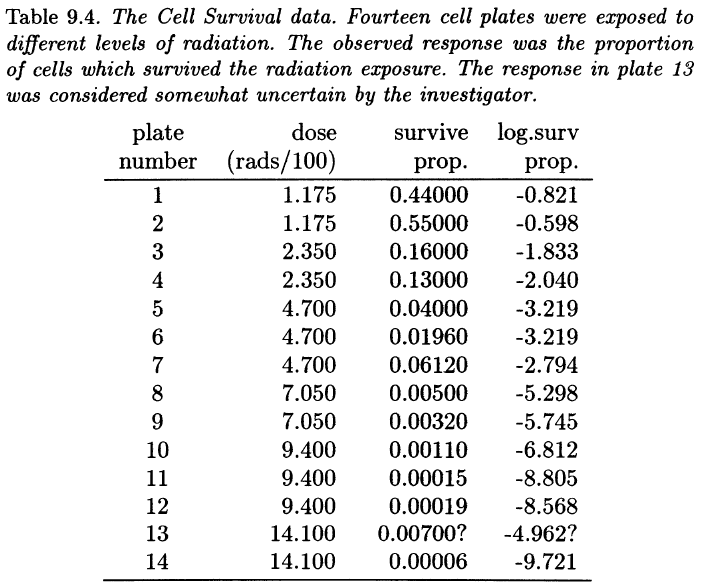
\includegraphics[width=\linewidth]{9/t94}
\newline
Отношение составляет $2.46$ для анализа, основанного на всех $14$ пластинах, что обычно считается убедительным доказательством того, что $\hat{\beta}_2$ значительно больше нуля. Если верить этому результату, то квадратичная модель (9.37) сильно предпочтительнее модели (9.36), которая имеет $\beta_2 = 0$.

Однако удаление сомнительной пластины $13$ из анализа снижает $\hat{\beta}_2/\widehat{\text{se}}(\hat{\beta}_j)$ только до $0.95$, что является незначимым результатом. Вывод заключается не в том, что $\beta_2$ \textit{обязательно} равен нулю, а в том, что он легко может быть равен нулю: если $\beta_2 = 0$, и если $(\beta_2) \dot = 0.0091$, как в строке 2 таблицы 9.5, то это вовсе не удивительно, что значение $\hat{\beta}_2$ такое же большое или больше наблюдаемого значения $0.0086$. Таким образом, у нас нет убедительных доказательств для отказа от линейной модели в пользу квадратичной модели.

Статистика --- это наука о сборе информации по крупицам с целью получения высокоинформативных сложных результатов. Статистики настораживаются, когда видят, что один элемент выборки, особенно подозрительный, доминирует в ответе на важный вопрос. Действительная критика регрессии по методу наименьших квадратов состоит в том, что один удаленный элемент, такой как пластина $13$, может иметь слишком большое влияние на подобранную кривую регрессии. Это показано на рисунке 9.3, на котором построена кривая регрессии методом наименьших квадратов как с пластиной $13$, так и без нее. Мощный эффект точки «?» очевиден.
\noindent
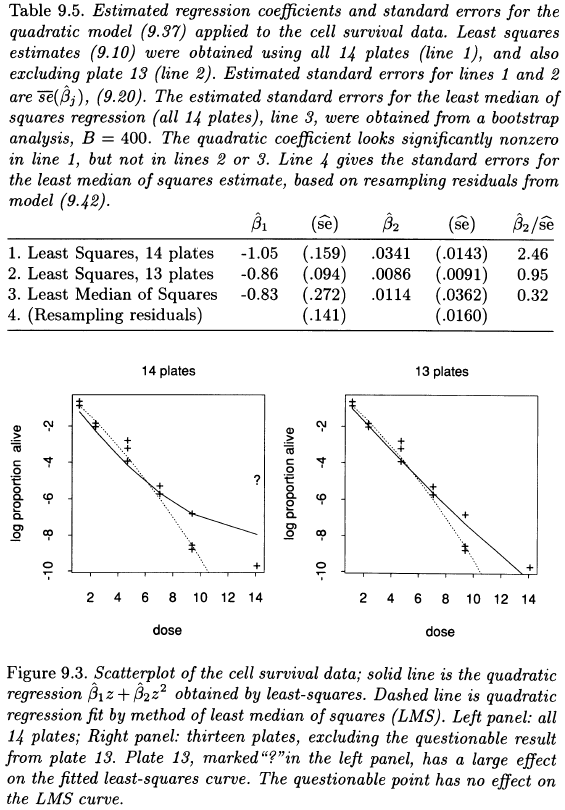
\includegraphics[width=\linewidth]{9/t95f93}
\newpage
\noindent Даже если бы исследователь не подвергал сомнению достоверность пластинки $13$, мы бы предпочли, чтобы наши подогнанные кривые не зависели так сильно от отдельных элементов выборки.